\section{Vérification}\label{sec:verification}

\subsection{Stratégie de test}

La vérification repose sur 77 tests \code{pytest} (environ 30~s sur la machine de mesure), répartis en cinq fichiers (tableau~\ref{tab:tests}). Le principe est de confronter chaque résultat à une référence \emph{indépendante} : une formule analytique, une autre méthode numérique ou une propriété physique.

\begin{table}[h]
\centering\footnotesize
\begin{tabular}{>{\ttfamily\footnotesize}l p{11cm}}
\toprule
\normalfont Fichier & Ce qui est vérifié\\
\midrule
test\_tangent.py & AD $=$ analytique ($<10^{-12}$) et DF $=$ analytique ($<10^{-7}$) pour 4 écrouissages $\times$ 3 états de déformation, avec ou sans pré-chargement ($\epsp$, $p$, $\X\neq0$) ; dérivée implicite $=$ dérivée à travers Newton ; symétrie de $\C^{ep}$ ; pas élastique $\Rightarrow\C$ ; piège $3\times3$.\\
test\_elastic\_limit.py & Petite déformation $\Rightarrow\sig=\C:\eps$ exactement ; courbe uniaxiale bilinéaire~\eqref{eq:Et} pour isotrope, cinématique et combiné ($10^{-10}$) ; coefficient de Poisson ; seuil à $\pm0{,}1\,\%$ de $\varepsilon_y$ ; $\tr\epsp=0$, $\X$ déviatorique, retour exact sur la surface ; décharge de pente $E$.\\
test\_pitfalls.py & Version naïve : \code{jacfwd} fini, \code{jacrev} NaN ; version sûre : aucun NaN en $\eps=\mathbf{0}$ dans les deux modes ; $\partial p/\partial\sigma_y$ fini et négatif ; \code{jit(vmap)} $=$ boucle $=$ NumPy ; FP32 préservé.\\
test\_driver.py & Linéaire proportionnel : 1 itération ; Voce : ordre empirique $>1{,}6$ ; tangente élastique : taux constant ; traction--cisaillement : 2 à 5 itérations.\\
test\_hyperelastic.py & $\Pk$ et $\mathbb{A}$ par AD $=$ formes analytiques (Neo-Hooke) ; symétrie majeure, $\Pk(\I)=\mathbf{0}$, objectivité $\Pk(\mathbf{Q}\F)=\mathbf{Q}\Pk(\F)$ ; invariants des essais ; Mooney--Rivlin uniaxial ; ICNN convexe et croissant.\\
\bottomrule
\end{tabular}
\caption{Contenu de la suite de tests.}\label{tab:tests}
\end{table}

\subsection{Précision de la tangente}

Le tableau~\ref{tab:tangent} donne l'écart relatif $\max|\C_X-\C^{ep}|/\max|\C^{ep}|$ pour un état fortement plastique (déformation multiaxiale, $p\approx2{,}5\times10^{-3}$).

\begin{table}[h]
\centering
\begin{tabular}{lcc}
\toprule
Écrouissage & AD / analytique & DF ($h=10^{-8}$) / analytique\\
\midrule
isotrope linéaire & $2{,}9\times10^{-16}$ & $4{,}2\times10^{-11}$\\
Voce & $2{,}9\times10^{-16}$ & $4{,}3\times10^{-11}$\\
Prager & $2{,}9\times10^{-16}$ & $4{,}5\times10^{-11}$\\
Voce + Prager & $2{,}9\times10^{-16}$ & $4{,}3\times10^{-11}$\\
\bottomrule
\end{tabular}
\caption{Écarts relatifs entre les trois tangentes.}\label{tab:tangent}
\end{table}

L'objectif du sujet ($10^{-12}$) est dépassé de quatre ordres de grandeur : l'AD et la formule analytique coïncident \emph{à l'arrondi machine près} ($\epsilon_{\mathrm{mach}}=2{,}2\times10^{-16}$). Ce n'est pas une coïncidence : l'AD calcule la même dérivée exacte que la dérivation à la main, seulement dans un ordre d'opérations différent.

\begin{figure}[h]
\centering
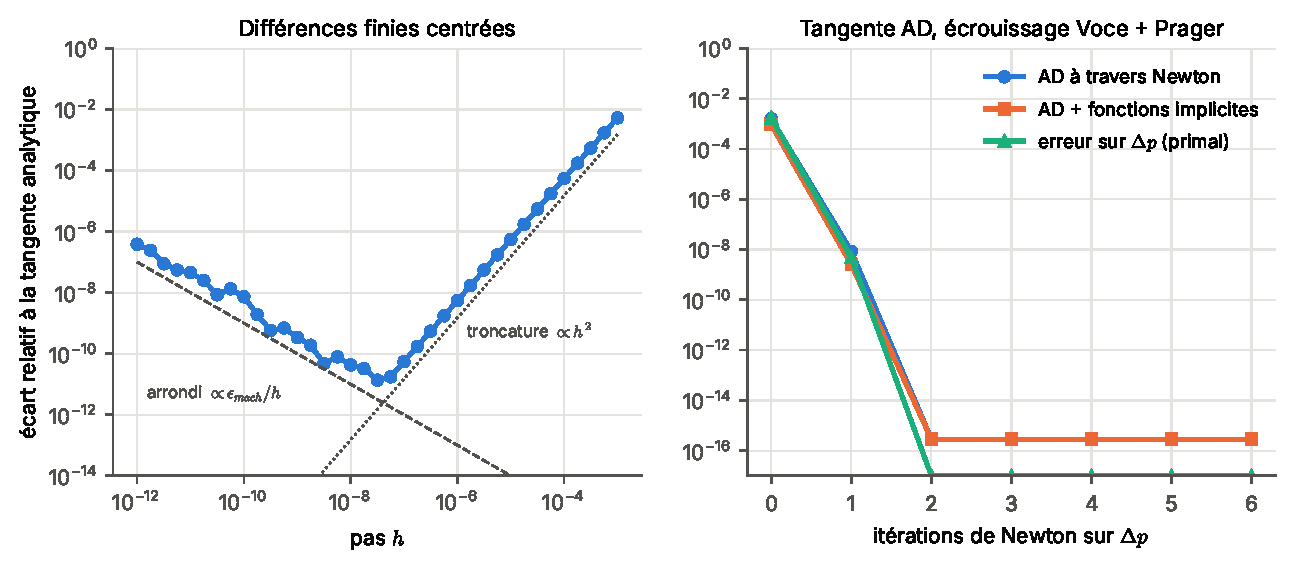
\includegraphics[width=\linewidth]{tangent_accuracy}
\caption{À gauche : erreur des différences finies centrées en fonction du pas $h$. On retrouve la courbe en V de la section~\ref{sec:df}, avec un optimum vers $h^\star\approx3\times10^{-8}$ et une erreur de $1{,}4\times10^{-11}$. À droite : erreur de la tangente AD en fonction du nombre d'itérations du Newton local sur $\Delta p$ (écrouissage Voce + Prager). Les deux modes de dérivation suivent l'erreur sur la solution primale et atteignent l'arrondi en 2 itérations.}\label{fig:tangent}
\end{figure}

\paragraph{Lecture de la figure~\ref{fig:tangent} (gauche).} Le pas optimal prédit est $h^\star\approx\epsilon_{\mathrm{mach}}^{1/3}\times|\eps|\approx6\times10^{-6}\times4\times10^{-3}\approx2\times10^{-8}$ et l'erreur minimale $\epsilon_{\mathrm{mach}}^{2/3}\approx4\times10^{-11}$. Les valeurs mesurées sont $3\times10^{-8}$ et $1{,}4\times10^{-11}$. Les différences finies sont donc une bonne vérification indépendante, mais pas un substitut à l'AD dans un code de production : elles coûtent 12 appels à la loi au lieu d'un, et donnent 5 chiffres de moins.

\paragraph{Lecture de la figure~\ref{fig:tangent} (droite).} L'initialisation $\Delta p^{(0)}$ laisse une erreur relative de $2\times10^{-3}$, qu'une itération réduit à $5\times10^{-9}$ et une deuxième à l'arrondi : c'est la convergence quadratique du Newton local. À 1 itération, la dérivée implicite ($2{,}6\times10^{-9}$) est un peu meilleure que la dérivée à travers les itérations ($8{,}5\times10^{-9}$). Au-delà, les deux sont exactes. Ici l'intérêt de la dérivation implicite n'est donc pas la précision. C'est la \emph{mémoire} en mode inverse et l'indépendance vis-à-vis de l'algorithme de résolution : on pourrait remplacer Newton par une bissection sans changer la dérivée.
